\documentclass[a4paper,11pt]{article}

\usepackage[latin1]{inputenc}
\usepackage[T1]{fontenc}
\usepackage{bbm} %math chars
\usepackage{amsmath}
\usepackage{indentfirst}
\usepackage{fullpage} %minimizes the default margins
\usepackage{url}
\usepackage{graphicx}
\usepackage[center,footnotesize]{caption} %options des legendes des graphes
\usepackage[section]{placeins} %place les figures d'une section avant le debut de la suivante
\usepackage{subfig} %a) b) c)
\usepackage{fancyvrb}

\title{Exercises - Week 13}
\date{}
\author{Genomics and bioinformatics}

\begin{document}
\maketitle

\section{Motif model}

\noindent The consensus is T \{C,T\} GA \{A,C,G,T\} \{A,T\}, or TYGANW using the IUPAC convention. 

\noindent The matrix $M$ is 

 
\begin{table}[h!]
\begin{center}
\begin{tabular}{|c|c|c|c|c|c|c|}
\hline
 & 1 & 2 & 3 & 4 & 5 & 6\\
\hline
A & 0 & 0 & 0 & 1 & 1/4 & 1/2\\
\hline
C & 0 & 1/2 & 0 & 0 & 1/4 & 0\\
\hline
G & 0 & 0 & 1 & 0 & 1/4 & 0\\
\hline
T & 1 & 1/2 & 0 & 0 & 1/4 & 1/2\\
 \hline
\end{tabular}
\end{center}
\end{table}

\noindent The information content is $I = (2, 1, 2, 2, 0, 1)$. The non-zero logo heights are: $\mbox{Height}_{T1} = 2$, $\mbox{Height}_{C2} = \mbox{Height}_{T2} = 1/2$, $\mbox{Height}_{G3} = 2$, $\mbox{Height}_{A4} = 2$, $\mbox{Height}_{A6} = \mbox{Height}_{T6} = 1/2$. The corresponding logo is\footnote{One can use http://weblogo.berkeley.edu/logo.cgi without the "Small Sample Correction" option.}

\begin{figure}[h!]
\centering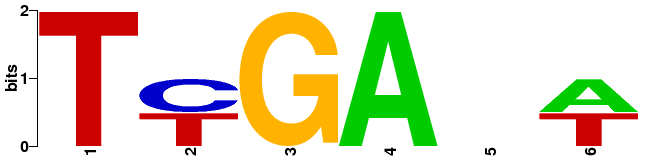
\includegraphics[width=9cm]{Logo.png}
\end{figure}

\section{Motif finding}

\noindent 1) The $N=10$ possible substrings of length $L=6$ are

\begin{figure}[h!]
\centering
\begin{BVerbatim}
ATTGAC
TTGACA
TGACAC
CCTTGA
CTTGAC
TTGACA
TTGACA
ATTGAC
TTGACA
TGACAC
\end{BVerbatim}
\end{figure}

\newpage
\noindent 2) The initial $10 \cdot M$ is

\begin{table}[h!]
\begin{center}
\begin{tabular}{|c|c|c|c|c|c|c|}
\hline
 & 1 & 2 & 3 & 4 & 5 & 6\\
\hline
A & 2 & 0 & 2 & 4 & 5 & 5\\
\hline
C & 2 & 1 & 0 & 2 & 4 & 5\\
\hline
G & 0 & 2 & 4 & 3 & 1 & 0\\
\hline
T & 6 & 7 & 4 & 1 & 0 & 0\\
 \hline
\end{tabular}
\end{center}
\end{table}

\noindent 3) The $N=10$ probabilities are 

\begin{eqnarray*}
p_1 = p_5 = p_8 = 2 \cdot 7 \cdot 4 \cdot 3 \cdot 5 \cdot 5 \cdot 1/10^6 &=& 4.2 \cdot 10^{-3}\\
p_2 = p_6 = p_7 = p_9 = 6 \cdot 7 \cdot 4 \cdot 4 \cdot 4 \cdot 5 \cdot 1/10^6 &=& 1.344 \cdot 10^{-2}\\
p_3 = p_{10} = 6 \cdot 2 \cdot 2 \cdot 2 \cdot 5 \cdot 5 \cdot 1/10^6 &=& 1.2 \cdot10^{-3}\\
p_4 = 2 \cdot 1 \cdot 4 \cdot 1 \cdot 1 \cdot 5 \cdot 1/10^6 &=& 4 \cdot 10^{-5}
\end{eqnarray*}

\noindent 4) We have 

$$
Const = \sum_{k=1}^N p_k = 3 \cdot 4.2 \cdot 10^{-3} + 4 \cdot 1.344 \cdot 10^{-2} + 2 \cdot 1.2 \cdot10^{-3} + 4 \cdot 10^{-5} = 0.0688~.
$$ 

\noindent The updated $Const \cdot M$ is

\begin{table}[h!]
\begin{center}
\begin{tabular}{|c|c|c|c|}
\hline
 & 1 & 2 & 3 \\
\hline
A & $p_1 + p_8$ & 0 & $p_3 + p_{10}$ \\
\hline
C & $p_4 + p_5$ & $p_4$ & 0  \\
\hline
G & 0 & $p_3 + p_{10}$ & $p_2 + p_6 + p_7 + p_9$ \\
\hline
T & $p_2 + p_3 + p_6 + p_7 + p_9 + p_{10}$ & $p_1 + p_2 + p_5 + p_6 + p_7 + p_8 +p_9$ & $p_1 + p_4 + p_5 + p_8$ \\
 \hline
\end{tabular}
\end{center}
\end{table}

\begin{table}[h!]
\begin{center}
\begin{tabular}{|c|c|c|c|}
\hline
 & 4 & 5 & 6\\
\hline
A & $p_2 + p_6 + p_7 + p_9$ & $p_1 + p_3 + p_5 + p_8 + p_{10}$ & $p_2 + p_4 + p_6 + p_7 + p_9$\\
\hline
C   & $p_3 + p_{10}$ & $p_2 + p_6 + p_7 + p_9$ & $p_1 + p_3 + p_5 + p_8 + p_{10}$ \\
\hline
G & $p_1 + p_5 + p_8$  & $p_4$ & 0\\
\hline
T  & $p_4$ & 0 & 0\\
 \hline
\end{tabular}
\end{center}
\end{table}

\noindent In summary, the updated $M$ is approximately 

\begin{table}[h!]
\begin{center}
\begin{tabular}{|c|c|c|c|c|c|c|}
\hline
 & 1 & 2 & 3 & 4 & 5 & 6\\
\hline
A & 0.12 & 0 & 0.03 &  0.78 & 0.22 & 0.78 \\
\hline
C & 0.06 & 0 & 0 & 0.03 & 0.78 & 0.22 \\
\hline
G & 0 & 0.03 & 0.78 & 0.18 & 0 & 0 \\
\hline
T & 0.82 & 0.96 & 0.18 & 0 & 0  & 0 \\
 \hline
\end{tabular}
\end{center}
\end{table}

\noindent 5) The consensus was TT \{G,T\} AA \{A,C\} and is now TTGACA, which was expected since TTGACA appears in each of the four binding sites. 

\end{document}











